\documentclass{scrreprt}

\usepackage{libertine}
\usepackage{graphicx}
\usepackage[table,xcdraw]{xcolor} %color in tables
\usepackage{hyperref}
\usepackage{array, tabularx, caption, boldline}
\usepackage{cellspace}
\usepackage{pdfpages} 
\usepackage{float}
\setlength\cellspacetoplimit{4pt}
\setlength\cellspacebottomlimit{4pt}
\usepackage{tikz}
\newcommand*\circled[1]{\tikz[baseline=(char.base)]{
		\node[shape=circle,draw,inner sep=2pt] (char) {#1};}}

\RedeclareSectionCommand[
  beforeskip=-.5\baselineskip,
  afterskip=.25\baselineskip]{subsubsection}
\RedeclareSectionCommand[
  beforeskip=-.5\baselineskip,
  afterskip=-0.5em]{paragraph}
\RedeclareSectionCommand[
  beforeskip=-.2\baselineskip,
  afterskip=-0.5em]{subparagraph}

\subject{EP Secure Cloud Energy Monitoring Platform WS 2018/19}
\title{Sprint 05 Security Report}
\subtitle{Scrum Master and Product Owner: Benedikt Holler \\ Author: Simonis Korbinian}
\author{Martin Binder\\Korbinian Simonis\\Benedikt Holler\\Andreas M\"uller\\Simon Sch\"onberger}
\date{As of \today}

\begin{document}
\maketitle
\section{Introduction}
\noindent In the following report, the results of a basic penetration test are presented. Since we have access to all the information (such as IPs, ports and the source code), it will be a white box test. Furthermore, only tests with low complexity are performed, since they are the most likely ones to occur and due to the short amount of given time. \\
The application runs on localhost, so no WAF or network property can influence the results.
Our penetration test is structured in four sections: \\
\begin{itemize}
	\item Information Gathering
	\item Vulnerability Analysis
	\item Exploitation
	\item Post Exploitation
\end{itemize} 

\paragraph{Information Gathering}
For our test scenario, active information gathering is the best method. The goal is to get as many informations of the host/web-application as possible. Therefore we enumerate and scan the open services, capturing ressources related to the application, review webpage metadata, identify application entry points etc. 

\paragraph{Vulnerability Analysis}
In this phase we aim to identify and evaluate the security risks posed by identified vulnerabilities.

\paragraph{Exploitation}
After finding a Vulnerability, we try to exploit it and gain access to the system. For this, tools like Metasploit are often used.

\paragraph{Post Exploitation}
In the Post-exploitation phase, we determine the value of the machine compromised and how to maintain control of the machine for later use with for example a backdoor or rootkit.

\pagebreak
\section{Information Gathering}

In this section we provide the results of our information gathering. As previous mentioned, we only use active information gathering.

\paragraph{nmap} 
("Network Mapper") is a free and open source (license) utility for network discovery and security auditing. It is mainly used for simple port scans, but also provides numerous scripts for security testing.
Our basic scan exposed just the port 8443, on which our application runs. Service detection failed, since it is not known by nmap. \\
An extended scan with usual vulnerability check scripts delivered more interesting results, shown in Figure \ref{nmap}.
\begin{figure}[h!]
	\centering
	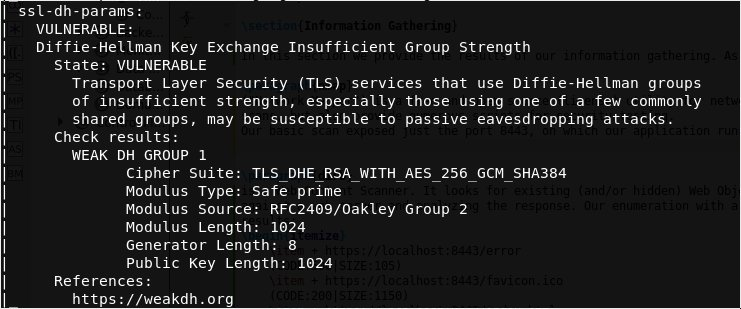
\includegraphics[width=15cm]{report/nmap_vul.jpg}
	\caption{Scan result of nmap}
	\label{nmap}
\end{figure}
\noindent This finding indicates that the SSL/TLS service uses Diffie-Hellman groups with insufficient strength; (key size less 2048). \\
\big[ \textit{Diffie–Hellman key exchange is a method of securely exchanging cryptographic keys over a public channel and was one of the first public-key protocols}.\big] \\
It was found that 1024 bits are breakable by really powerful attackers like the NSA. For our prototype it may be sufficient, but in real life use at least 2048, better 4096 bits should be chosen.

\paragraph{dirb}
is a Web Content Scanner. It looks for existing (and/or hidden) Web Objects. It basically works by launching a dictionary based attack against a web server and analyzing the response. Our enumeration with a standard wordlist of common directory names provided following results: 
\begin{itemize}
	\item + https://localhost:8443/error (CODE:500|SIZE:105)                                                                                                                                                                
	\item + https://localhost:8443/favicon.ico (CODE:200|SIZE:1150)                                                                                                                                                         
	\item + https://localhost:8443/index.html (CODE:200|SIZE:2590)                                                                                                                                                          
	\item + https://localhost:8443/logout (CODE:302|SIZE:0)       
\end{itemize}

\noindent Each finding has been manually examined for possible security concerns, but nothing relevant or alarming was found.

\section{Vulnerability Analysis}
 
For the Vulnerability Analysis, we performed automated as well as manual tests to cover as wide a spectrum as possible.

\subsection{Automated Scans}
\paragraph{Nikto}
is an Open Source (GPL) web server scanner which performs comprehensive tests against web servers for multiple items, including over 6700 potentially dangerous files/programs, checks for outdated versions of over 1250 servers, and version specific problems on over 270 servers. It also checks for server configuration items such as the presence of multiple index files, HTTP server options, and will attempt to identify installed web servers and software. Scan items and plugins are frequently updated and can be automatically updated.
\begin{figure}[h!]
	\centering
	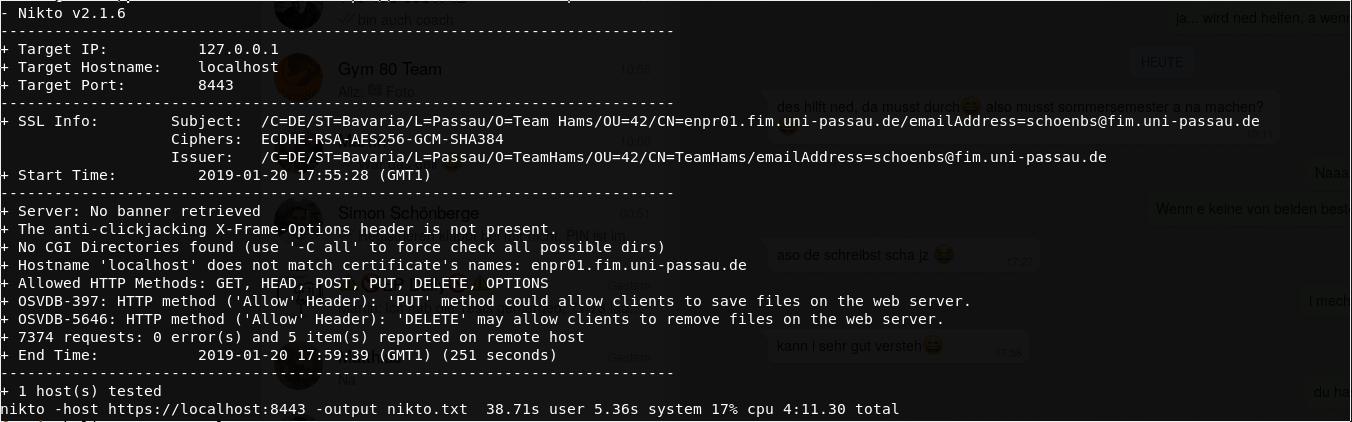
\includegraphics[width=15cm]{report/nikto.png}
	\caption{Scan result of Nikto scanner}
	\label{nikto}
\end{figure}

\noindent The only relevant vulnerability nikto found is the missing anti-clickjacking X-Frame options header, which may allow possible attackers to clickhijack under certain circumstances. \\
\big[ \textit{Clickjacking, also known as a "UI redress attack", is when an attacker uses multiple transparent or opaque layers to trick a user into clicking on a button or link on another page when they were intending to click on the the top level page}.\big] \\
Additionally, the scan provides some useful information about a potential admin/user of the application, since in the ssl info an email address of the company is included.

\paragraph{Owasp-zap}
(short for Zed Attack Proxy) is an open-source web application security scanner. Even though the application is intended as a proxy, it offers many other possibilities such as security scans, webspider, fuzzering and much more. Figure \ref{zap} shows a summary of the scan results. We have only one alert with a medium risk level. Figure \ref{zap1} shows more details on the finding. Again, it is the missing anti-clickjacking X-Frame options header. 
\begin{figure}[h!]
	\centering
	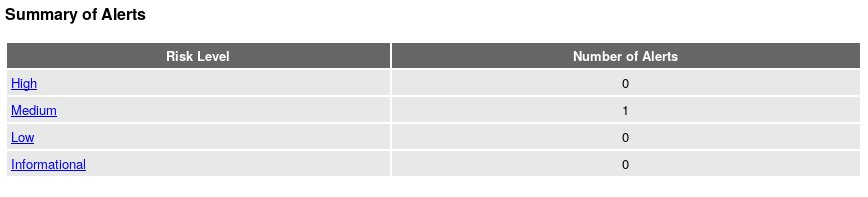
\includegraphics[width=15cm]{report/owasp0.jpg}
	\caption{Owasp zap scan summery}
	\label{zap}
\end{figure}

\begin{figure}[h!]
	\centering
	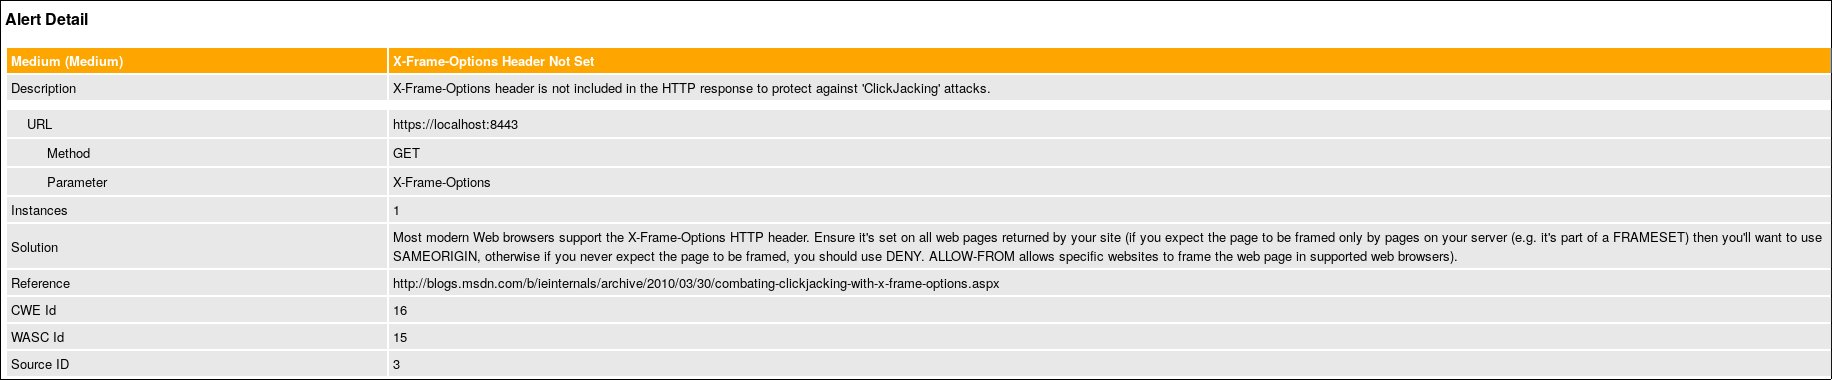
\includegraphics[width=17cm]{report/owasp.jpg}
	\caption{Owasp zap alert detail}
	\label{zap1}
\end{figure}


\subsection{Web Proxy Testing}

In this subsection, we use Burp Suite, a graphical tool for testing Web application security, with the main purpose to serve as a http proxy. Figure \ref{request} shows a login request captured with burp. This request is later used for the sql injection and the brute force attack, as well as for the Session Testing.

\subsubsection{Session Testing}
 In this subsubsection, we perform several test to check if the session ids/ jwt access tokens are reacting as expected after manipulation.

\begin{figure}[h!]
	\centering
	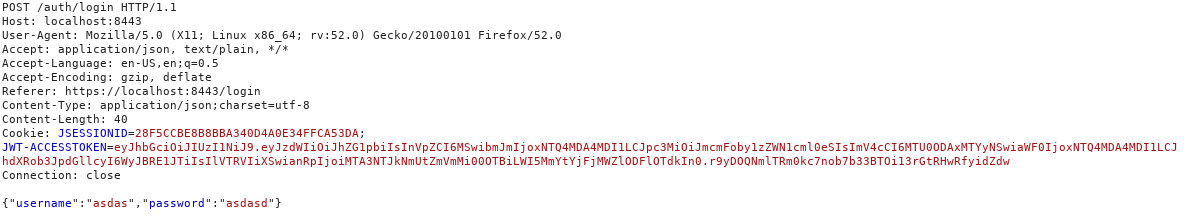
\includegraphics[width=17cm]{report/log.png}
	\caption{Captured login request with burp proxy}
	\label{request}
\end{figure}

\paragraph{Test 01:} Manipulating the jsessionid \\
The purpose of this test is to check, if after manipulation of the jsession id, the request is still valid and gets the requested content. We test with two types of manipulation, on the one hand a random jsessionid in valid format, on the other hand a random character sequence. \\
We expect that the request is invalid after any change to the jsessionid.
In concrete, we login with admin credentials and request the 'Node settings' page of our EMS. We modify then with burp the jsessionid and send the request again.\\
The response of both test types is depicted in Figure \ref{session02}, so the behavior is as expected. 

\begin{figure}[h!]
	\centering
	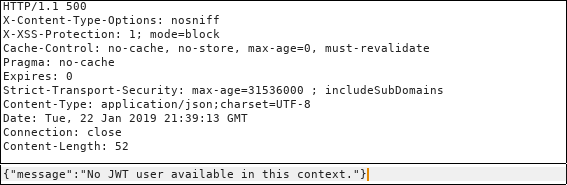
\includegraphics[width=14cm]{report/session02.png}
	\caption{Response of request with changed jsessionid}
	\label{session02}
\end{figure}

\paragraph{Test 02:} Manipulating the jwt-accesstoken \\
Basically the same as in \textbf{Test 01}, but here we manipulate the jwt-accesstoken, instead of the jsessionid.
Again, we expect, that requests with the manipulated tokens are invalid. Our tests could confirm this, as shown in Figure \ref{session03}.

\paragraph{Test 03:} Logout test \\
In this test we want to verify that after a logout the jsessionid is useless. \\
Again, we capture the get request for the 'node settings' and try to access the content after a logout. Expected behavior is, that the jsessionid is invalid after a logout and all following request with this id will fail. \\
The initial tests failed, further explanations can be found in the following paragraph.
\begin{figure}[h!]
	\centering
	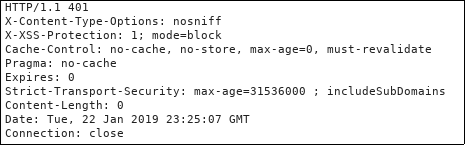
\includegraphics[width=14cm]{report/session03.png}
	\caption{Response of request with changed jsessionid}
	\label{session03}
\end{figure}

\pagebreak
\paragraph{Bugfix Test 01/02/03}
In the previous tests a bug was found, which was due to the use of the h2 profile in the build. Since we use a stateless connection, there should be no jsessionid. In Figure \ref{session04}, a request without the incorrect jsessionid is depicted. Now if you manipulate the jwt-accesstoken in any way, the request will be invalid. After a logout, the token will be valid until it expires, but this is to the best of our knowledge intended by design and no bug.
\begin{figure}[h!]
	\centering
	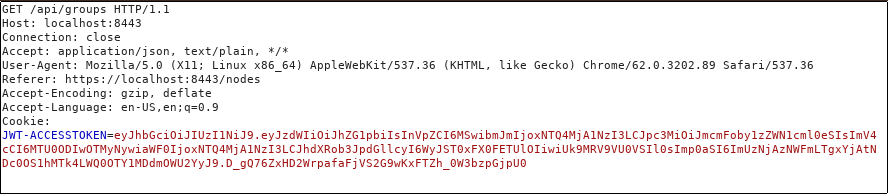
\includegraphics[width=14cm]{report/session04.png}
	\caption{Correct request without jsessionid}
	\label{session04}
\end{figure}


\pagebreak 

\subsection{Encryption Verification}
\paragraph{Wireshark}
is a free and open-source packet analyzer. It is used for network troubleshooting, analysis, software and communications protocol development.
In our test scenario we use it to check whether all packages are encrypted. Figure \ref{wire} shows a captured encrypted login request with wireshark. The same request is depicted in Figure \ref{wire0}, but here no TLS is used, so an attacker could easily extract the login credentials from it. This way, we have captured and reviewed several tcp streams of sample user interactions. Furthermore, critical interactions such as the registration of a new node were also examined.
\begin{figure}[h!]
	\centering
	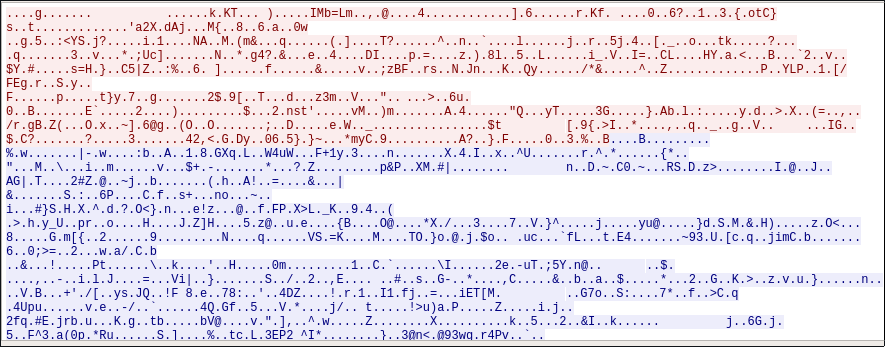
\includegraphics[width=17cm]{report/wire_login_ssl.png}
	\caption{Captured encrypted login request with wireshark}
	\label{wire}
\end{figure}
\begin{figure}[h!]
	\centering
	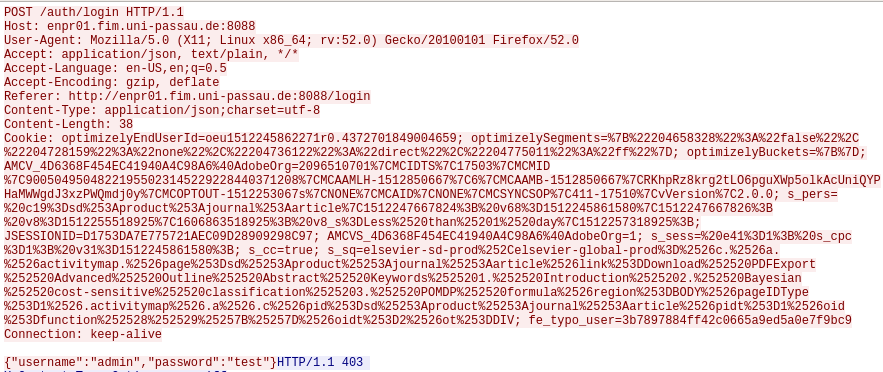
\includegraphics[width=17cm]{report/wire_login_.png}
	\caption{Captured plaintext login request with wireshark}
	\label{wire0}
\end{figure}


\subsection{SQL Injection Testing}
\paragraph{SQLMap} is an open source penetration testing tool that automates the process of detecting and exploiting SQL injection flaws and taking over of database servers. For our application, we have used an aggressive scan that poses a high risk of being discovered. The reasons for this are a higher chance of success. In a real life scenario, the WAF would most likely block the requests from a certain point in time like shown below. \\
\textit{[00:09:20] [CRITICAL] previous heuristics detected that the target is protected by some kind of WAF/IPS} \\
\textit{[00:12:03] [WARNING] there is a possibility that the target (or WAF/IPS) is dropping 'suspicious' requests} \\
Since in our application all SQL querries are handled by Spring Boots repository, it was assumed that there are no trivial injection possibilities. SQLmap has confirmed this assumption, all scans performed found no vulnerability.


\section{Exploitation}
Since no real vulnerability was found, the only simple attack to perform was brute forcing the login page.

\paragraph{Login Bruteforce}
With the previous captured login request, we were able to brute force the login with the intruder module of burp. The username was guessed, since it is most common to use 'admin' for web applications. Our previous with nikto discovered possible username was not useful here. Figure \ref{brute} shows the successfull payload. We used a standard wordlist for the attack. Although this is not a real software vulnerability, bad password policy is a very common attack vector.
\begin{figure}[!h]
	\centering
	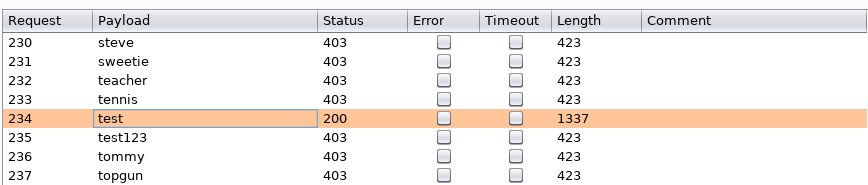
\includegraphics[width=14cm]{report/brute.jpg}
	\caption{Extract from Burpsuite's intruder}
	\label{brute}
\end{figure}
Brute forcing was only possible since a very weak password from the development phase was accidentally taken over into the live application. By using bcrypt with a sufficiently high iteration count, a strong password is probably only obtainable over a very long period of time, so that this kind of attack is not realy promising.

\pagebreak
\section{Post Exploitation}
In this phase, we mainly tried with the found credentials to create a permanent access to the software, without being noticed. For this we tried to create another admin user. [Result]
Furthermore, an attempt was made to get access to the underlying VM from the application. Usually, this is most easily done by remote code execution (RCE). Often, these vulnerabilities are found in the application upload options, where the website is tricked to run for example PHP code and to open a reverse shell. But since no upload possibilities were found and all input fields were checked for command execution, an attacker will not be able to gain access to the system without a more complex form of exploit.

\section{Summary}
In this section a short summary of the results is provided. \\

\noindent In our info \textbf{gathering phase}, we initialy performed a port scan with nmap to discover open ports and services. In our case just port 8443 is relevant, the service detection failed, since nmap did not recognize our application. The additional scan with the default vulnerability scripts, provided a weak cipher key lenght, but nothing to exploit without very strong computing power. 
Also, we were able to uncover some additional pages, but these did not provide any further useful information. \\
The \textbf{vulnerability analysis} phase started we automated scans of nikto and owasp-zap. Both found a anti-clickjacking X-Frame options header of medium risk level. But due to the lack of time, we could not refer to it. Nikto also found a valid email address in the ssl info, which could have lead to a user or admin account of the application. After that, we used burp proxy to capture requests of user interactions with the software and checked the jwt-accesstoken behavior. After extensive bugfixing, the tokens now behave like expected. The next step we performed, was to verify encryption of the send packages. Here we used wireshark and could confirm encryption. We also tested several input field for SQL injection with sqlmap, but we could not find any vulnerabilities, which is probably due to the fact, that our sql queries are automatically generated by spring and a weakness here is not very likely.
Since we did not find any promising vulnerabilities, we had nothing realy to exploit in the \textbf{exploitation} phase. That is why we tried to brute force the login page and could this way find the admin credentials, which was only possible due to a very bad password policy. With this credentials we examined in the last phase, the \textbf{post exploitation} phase, the application for possible RCE weaknesses, but nothing was found. \\
Overall, no serious vulnerabilities were found.   
\end{document}

